\chapter{Introduction}
\label{cha:introduction}


\section{Motivation}

\begin{center}
    \includegraphics[width=\textwidth]{mensa}\\
    The mensa in Hardenbergstraße at TU Berlin.
\end{center}

\begin{center}
    \includegraphics[width=\textwidth]{use-case-mensa-people}\\
    Yellow person looking for her/his friends in crowded mensa.
\end{center}

\begin{center}
    \includegraphics[width=\textwidth]{use-case-tablet}\\
    Imagined use of our app on mensa tray.
\end{center}

\begin{center}
    \includegraphics[width=\textwidth]{user-story}\\
    Steps on user's way to her/his friends.
\end{center}


\section{Constraints}

The idea of this project described above already introduced some implicit constraints in order to make it work. To have a complete overview of what we expect to have available to use our service, we defined the following constraints:

\begin{itemize}
    \item \textbf{Everyone has a smartphone}: Obvious point. As this project involves developing clients for Android and iOS and relying on these clients to interact in an user friendly manner with the backend, a smartphone is needed. We do not, though, require the latest operating system versions. For Android, version 5.0 is required, for iOS, version X is required.
    \item \textbf{Participants have a TUB account (edugain account)}: The service we provide needs an authentication prior to being able to modify or delete objects on backend side. Therefore some kind of user management was needed. As we will explain more deeply later in this document, for user authentication and session management we rely on a department service called CYCLONE Federation Provider\footnote{\url{http://www.cyclone-project.eu/}}. Via this service users with an edugain (and therefore a TUB) account are able to authenticate against our backend.
    \item \textbf{Minimal interaction}: As described in the previous section our intended use case is placed in situations where you probably carry a tray full of food and will not be having your hands free to interact with complex user interfaces. Therefore a very important constraint for our project was to provide applications that do not need a lot of intention in order to work as intended while at the same time striclty comply with the user's set preferences.
    \item \textbf{Easy to use}: This constraint correlates with the previous one. The setting our applications are intended for do not allow for complex user interfaces. Actions needed to be taken while using the services need to be easy to perform.
    \item \textbf{Low impact on device battery}: The possible use of bluetooth introduced the topic of battery usage. We therefore defined low battery usage as an important constraint for our project.
\end{itemize}


\vspace{0.5cm}

\section{Functional Requirements}

After motivation and constraints were set, we defined our functional requirements. These were the functions we had to implement to follow along our imagined flow throughout the application. Therefore a user has to be able to\ldots

\begin{itemize}
    \item \textbf{\ldots login via university account}: As mentioned in our constraints, login should happen via the university account. We are using the CYCLONE Federation Provider and therefore things work a little different than in a self-developed login mechanism. For us this meant to integrate the provided OpenID Connect authentication flow in a user friendly way into the mobile applications. The applications in turn would then be authenticated against the backend.
    \item \textbf{\ldots add friends via university mail}: All connected edugain members each have their own unique domain name and internally only contain unique users. It was the logical step to provide the functionality to add friends by their mail address as the unique identifier.
    \item \textbf{\ldots share her/his location}: The most important part of our system is the modifiability of the logged in user only. This includes updating or deleting the user's location and defining in which conditions and with which friends the location should be shared.
    \item \textbf{\ldots see shared locations of friends}: Friends' locations were supposed to be visualized on a map. To realise this a functionality to retrieve locations of friends directly in the user's area needed to be developed.
\end{itemize}